%------------------------------------------------------------------------------------------
% HOW TO COMPILE THIS DOCUMENT WITH TEXMAKER:  
% 1. Run BibTeX (F11)
% 2. Run MakeIndex (F12)
% 3. Run Quickbuild or equivalent (F1)
%
% Sometimes, a second or third cycle is required to get all references right. 
%------------------------------------------------------------------------------------------

% Festlegung des Allgemeinen Dokumentenformats
\documentclass[a4paper,table,10pt]{article}

% Layout anwenden
\usepackage{latex_einstellungen/layout}

%------------------------------------------------------------------------------------------
% BEGIN OF DOCUMENT
%------------------------------------------------------------------------------------------
\begin{document}
% hier werden die Trennvorschläge inkludiert
%hier müssen alle Wörter rein, welche Latex von sich auch nicht korrekt trennt bzw. bei denen man die genaue Trennung vorgeben möchte
\hyphenation{
Soft-ware-bau-steins
Dem-ent-sprech-end
}


% Deckblatt
\thispagestyle{empty}
 
\begin{flushleft}
\smallskip
\end{flushleft}

\begin{flushleft}
\vspace{10 mm}
\textbf{{\fontsize{35}{20}\selectfont {\titleDocument}}}
\end{flushleft}

\begin{flushleft}
\bigskip
\bigskip
\end{flushleft}

\begin{flushleft}
\documentAuthor
\vspace{40 mm}
\end{flushleft}


\begin{flushleft}
\textbf{{\fontsize{20}{20}\selectfont {\subjectDocument}}}
\end{flushleft}

\vspace{2 mm}

\begin{figure}[h!]
 \centering
 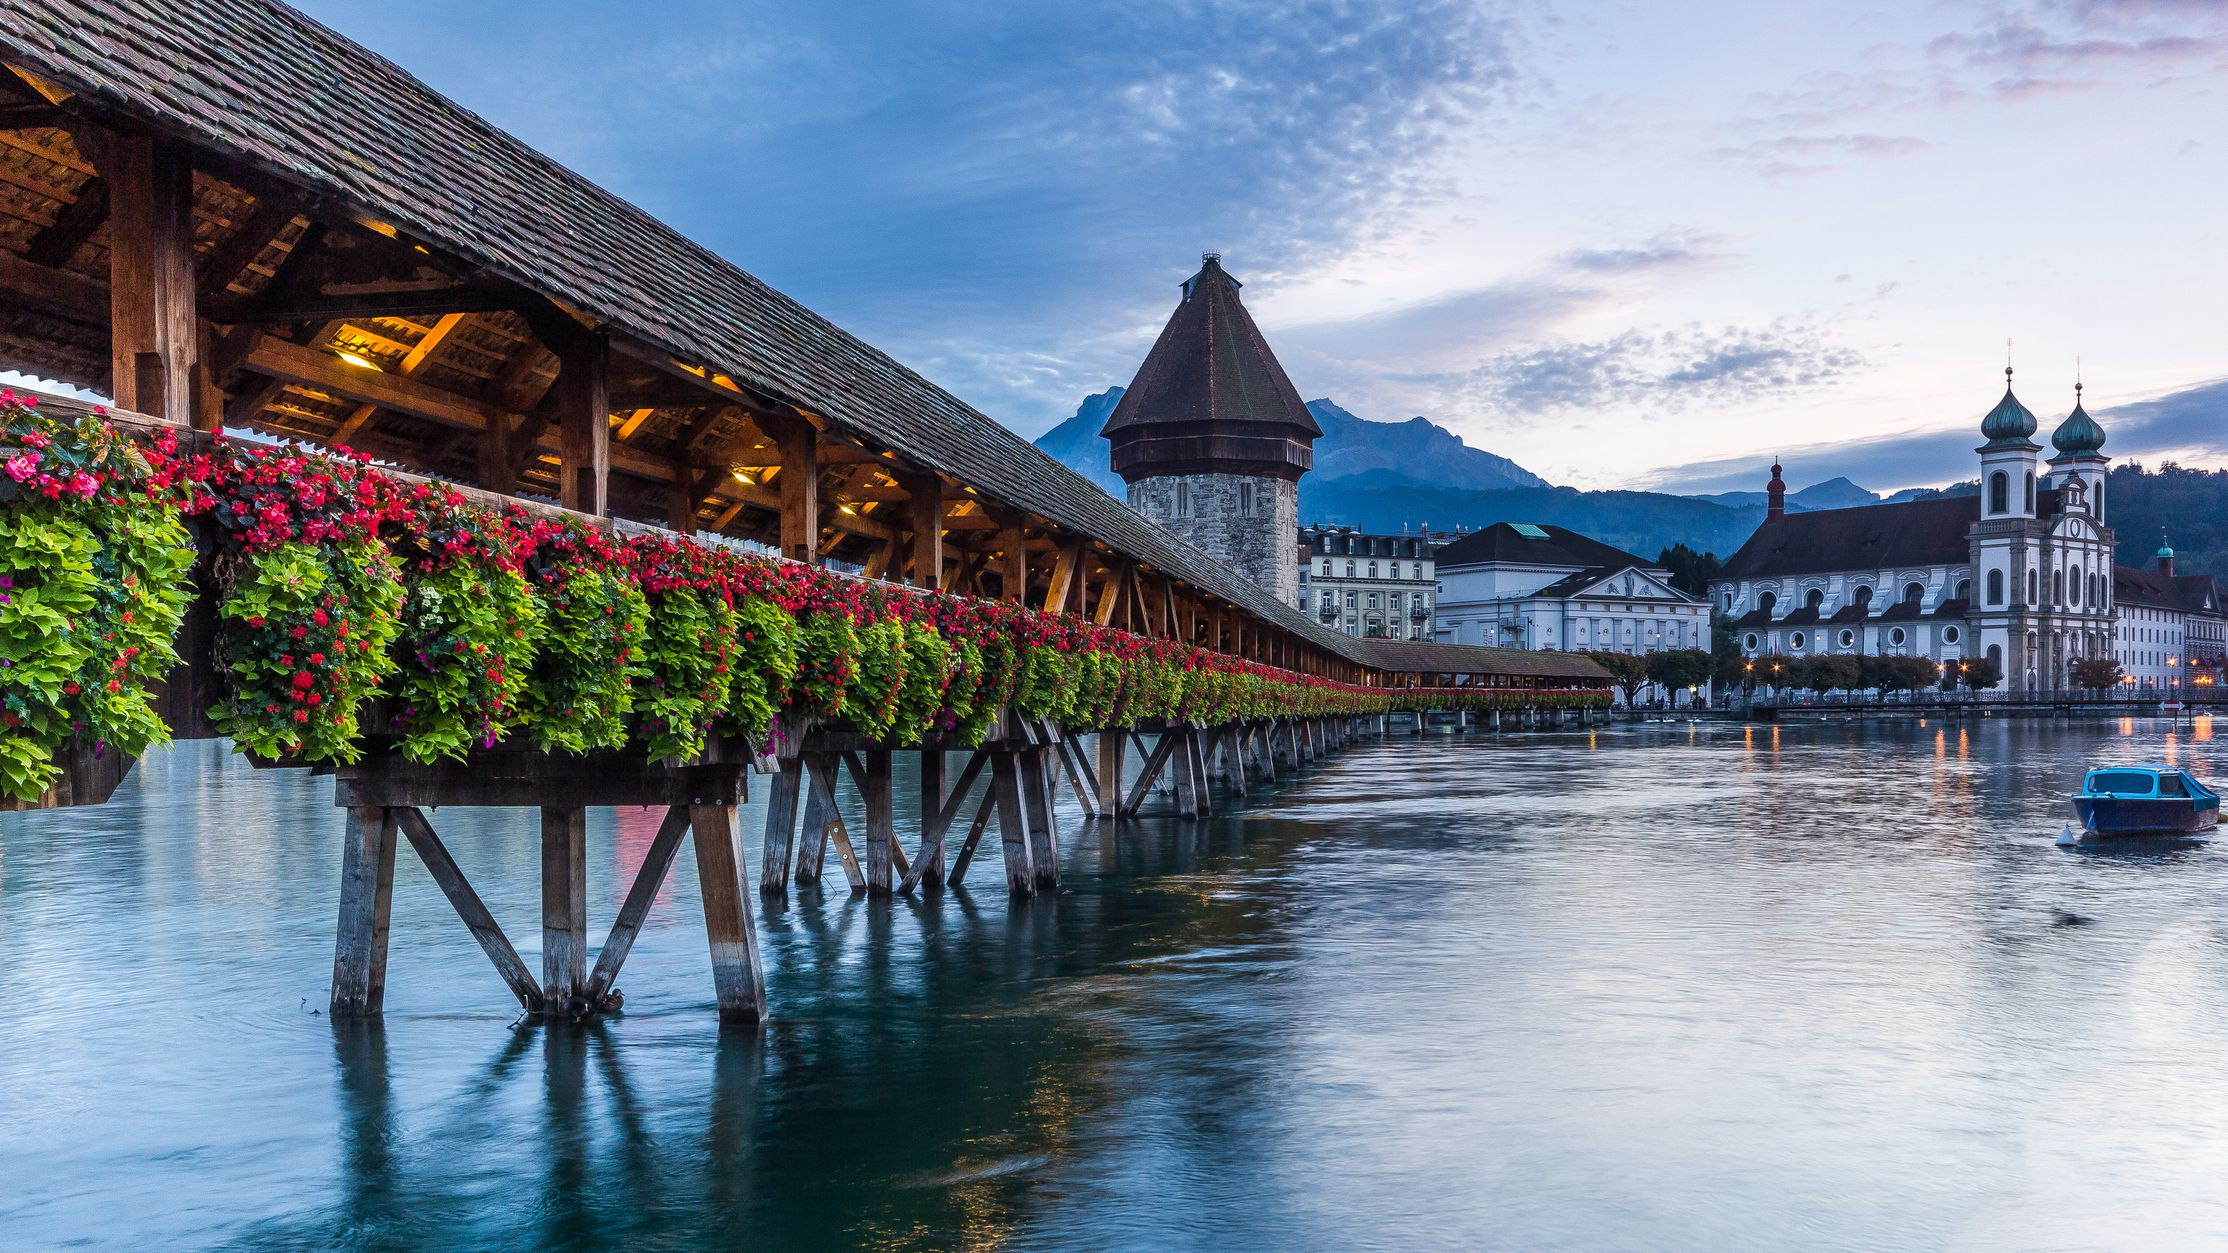
\includegraphics[width=0.9\textwidth]{../fig/placeholder}
\end{figure}

\vfill


\begin{flushleft}
\institutionNameLong \\
\titleDocument\ (\moduleAbbreviation) \\
\end{flushleft}

\begin{flushleft}
\institutionLocation, \institutionNameShort, \today\\
\end{flushleft}


\pagebreak
\thispagestyle{empty} % erzeugt Seite ohne Kopf- / Fusszeile
\mbox{}
\newpage
\pagebreak

% 1.5 facher Zeilenabstand
\onehalfspacing

% Titelblatt
\begin{titlepage}
\pagestyle{completelyEmpty}
\includepdf[pages=-,pagecommand={}]{titelblatt/titelblatt_hslu.pdf}
\end{titlepage}

% einfacher Zeilenabstand
\singlespacing

%------------------------------------------------------------------------------------------
% DIVERSE VERZEICHNISSE
%------------------------------------------------------------------------------------------
% Inhaltsverzeichnis anzeigen
\tableofcontents

% Abbildungsverzeichnis
\newpage
% Abbildungsverzeichnis soll im Inhaltsverzeichnis auftauchen
\rhead{\emph{Abbildungsverzeichnis}}
\addcontentsline{toc}{section}{Abbildungsverzeichnis}
\listoffigures

% das Tabellenverzeichnis
\newpage
% Tabellenverzeichnis soll im Inhaltsverzeichnis auftauchen
\rhead{\emph{Tabellenverzeichnis}}
\addcontentsline{toc}{section}{Tabellenverzeichnis}
% Tabellenverzeichnis endgültig anzeigen
\listoftables

% Abkürzungsverzeichnis
\newpage
% Abkürzungsverzeichnis soll im Inhaltsverzeichnis auftauchen
\section*{Abkürzungsverzeichnis}\label{sec:abkuerzungsverzeichnis}
\rhead{\emph{Abkürzungsverzeichnis}}
\begin{acronym}[1234567]	% Längste Abkürzung in [] platzieren für Längenbestingung des Abstandes
	\acro{ADC}{Analog-to-digital converter\acroextra{\textit{, dt. = Analog-zu-Digital Umwandler}}}
	\acro{BAT}{Bachelor-Thesis}
%Falls eine Abkürzung in der Mehrzahl nicht einfach auf "s" endet muss das speziell eingestellt werden. 
% \acro{slmtA}{super lange mega tolle Abkürzung} %Einzahl
% \acroplural{slmtA}[slmtAs]{super lange mega tolle Abkürzungen} %Mehrzahl
\end{acronym}

%------------------------------------------------------------------------------------------
% KAPITEL 1 ff. 
%------------------------------------------------------------------------------------------
\newpage
\onehalfspacing		% 1,5 facher Zeilenabstand

% einzelne Abschnitte
\rhead{\emph{Schrift oben rechts}}
\section{Hauptkapitel}\label{sec:hauptkapitel}
Beispielsdokument (\emph{bzw. Vorlage}) für eine \ac{BAT}\footnote{Bei Mehrzahl kann apc statt ac verwendet werden.}. Es folgt ein Zeilenumbruch.\\ 
~\\ % leere Zeile
Ich bin ein Quellenverweise, gesehen in \cite[S.~57]{KeilStefan2017D}. Ein Text in "'Anführungszeichen"'.\\\\
\lipsum[1]
\begin{figure}[H]
	\centering
	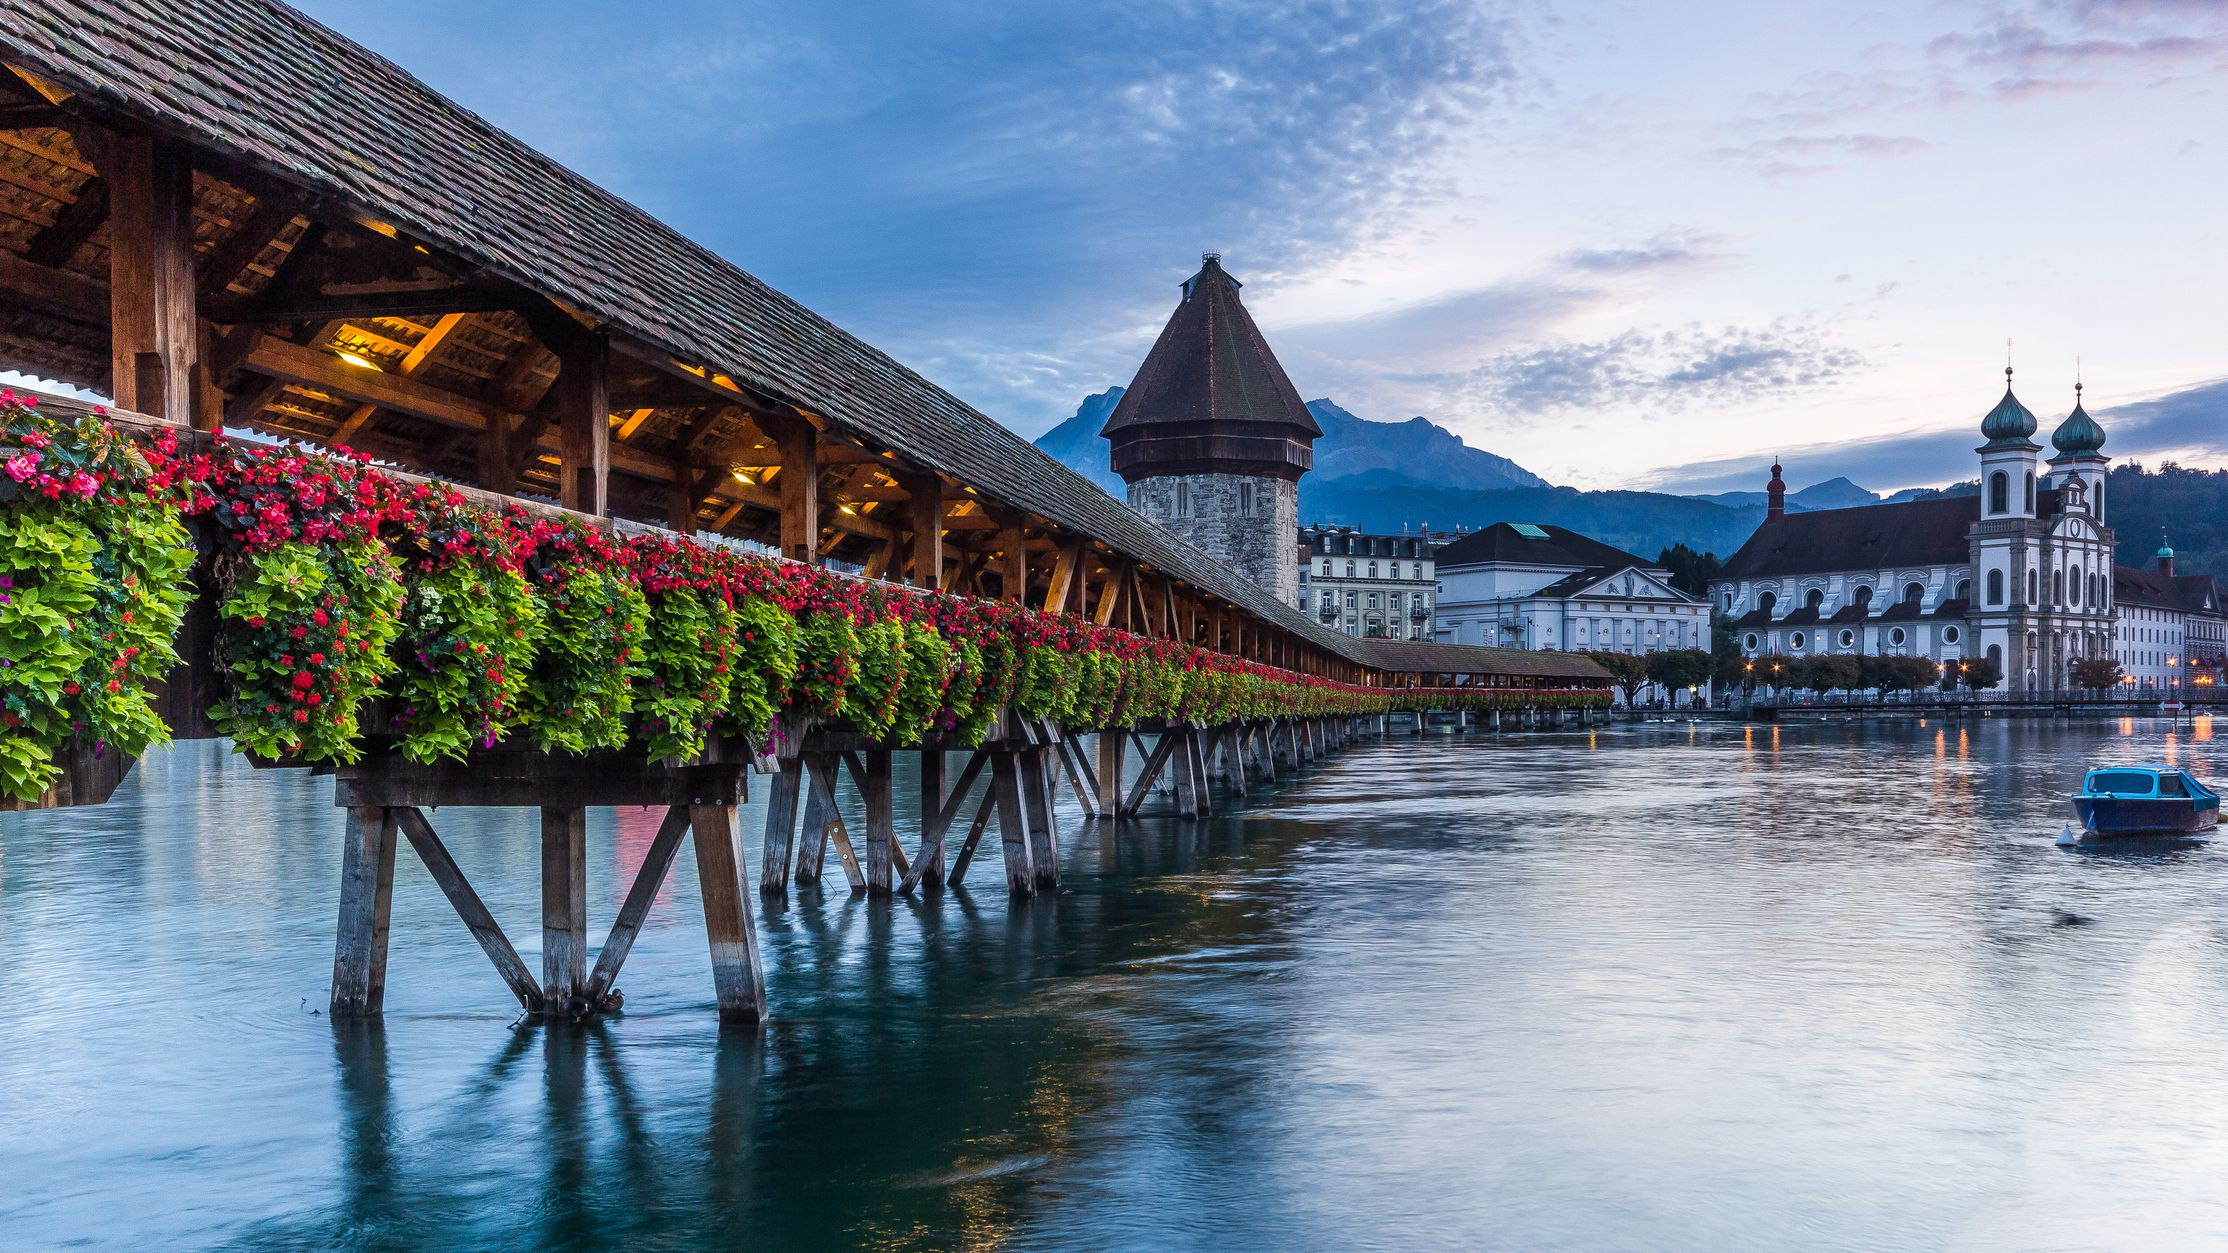
\includegraphics[width=0.75\textwidth]{../fig/placeholder}
	\caption{Platzhalter für ein Bild}
	\label{fig:testaufbau_uebersicht}
\end{figure}
\subsection{Unterkapitel}
\lipsum[1]\\\\
Es folgt ein Seitenumbuch.
\newpage \noindent
\textbf{Nicht nummerierte Aufzählung:}
\begin{itemize}[itemsep=-5pt,topsep=0pt]
	\item Element 1 einer Aufzählung
	\item Element 2 einer Aufzählung
	\begin{enumerate}[a), itemsep=-2pt,topsep=-6pt]
		\item Unterelement von 2 
		\item Ebenso
	\end{enumerate}
	\item Element 3 einer Aufzählung
\end{itemize}
\textbf{Nummerierte Aufzählung:}
\begin{enumerate}[itemsep=-5pt,topsep=0pt]
	\item Element 1 einer Aufzählung
	\item Element 2 einer Aufzählung
	\item Element 3 einer Aufzählung
\end{enumerate}
\subsubsection{Unterunterkapitel}
Zwei Bilder nebeneinander.
\begin{figure}[H]
	\centering
	\captionsetup[subfigure]{justification=centering}
	\begin{subfigure}[b]{0.48\textwidth}
  	\centering
		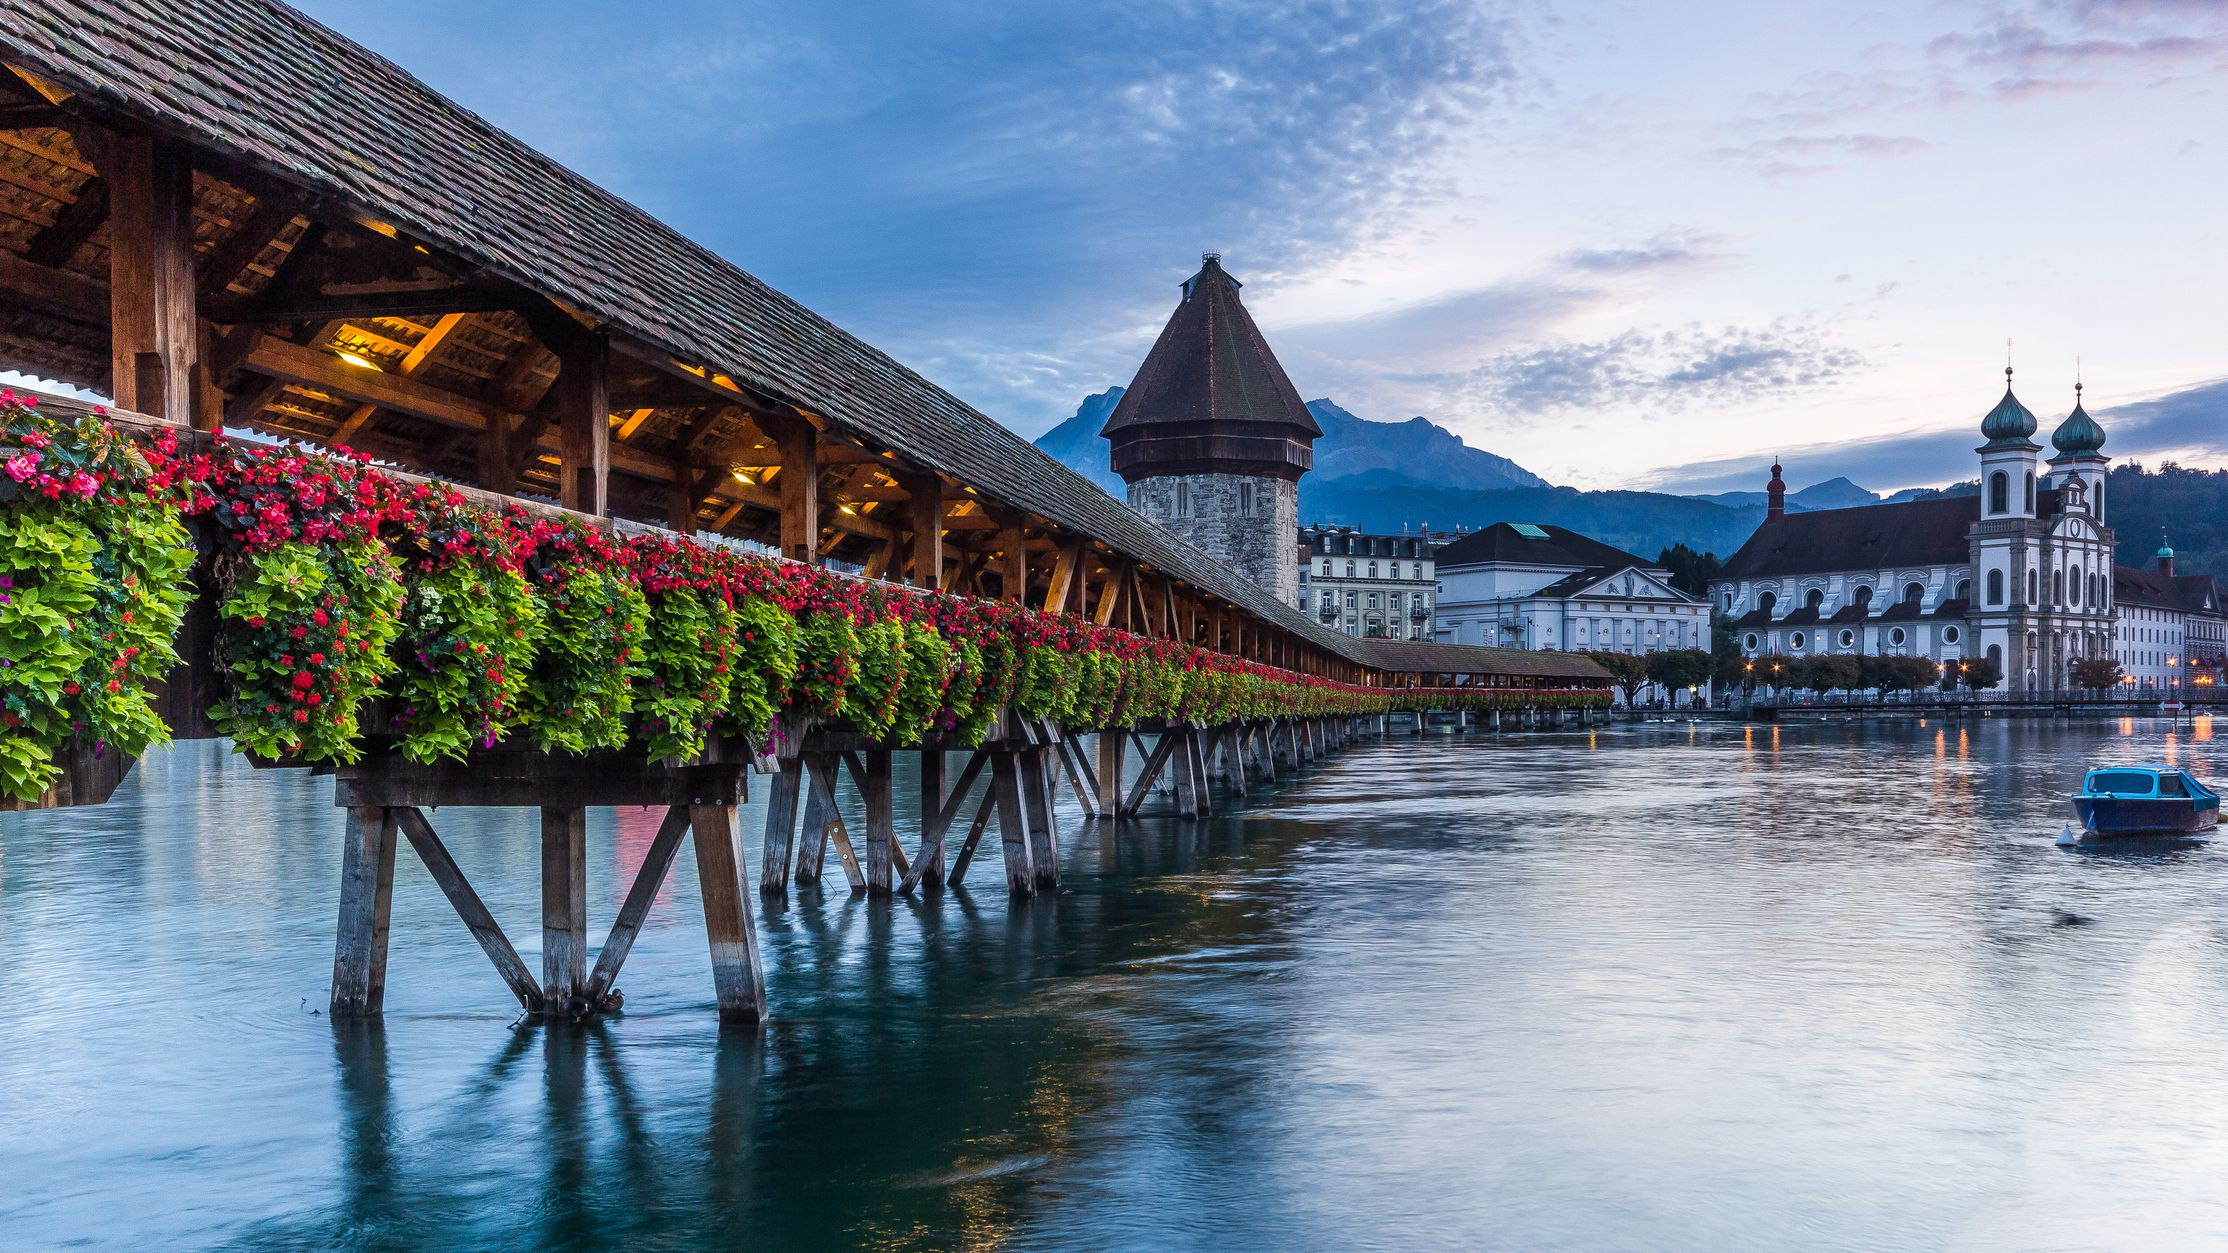
\includegraphics[width=0.95\linewidth]{../fig/placeholder}
		\caption{Bild links}
		\label{fig:left}
	\end{subfigure}
	\begin{subfigure}[b]{0.48\textwidth}
		\centering
		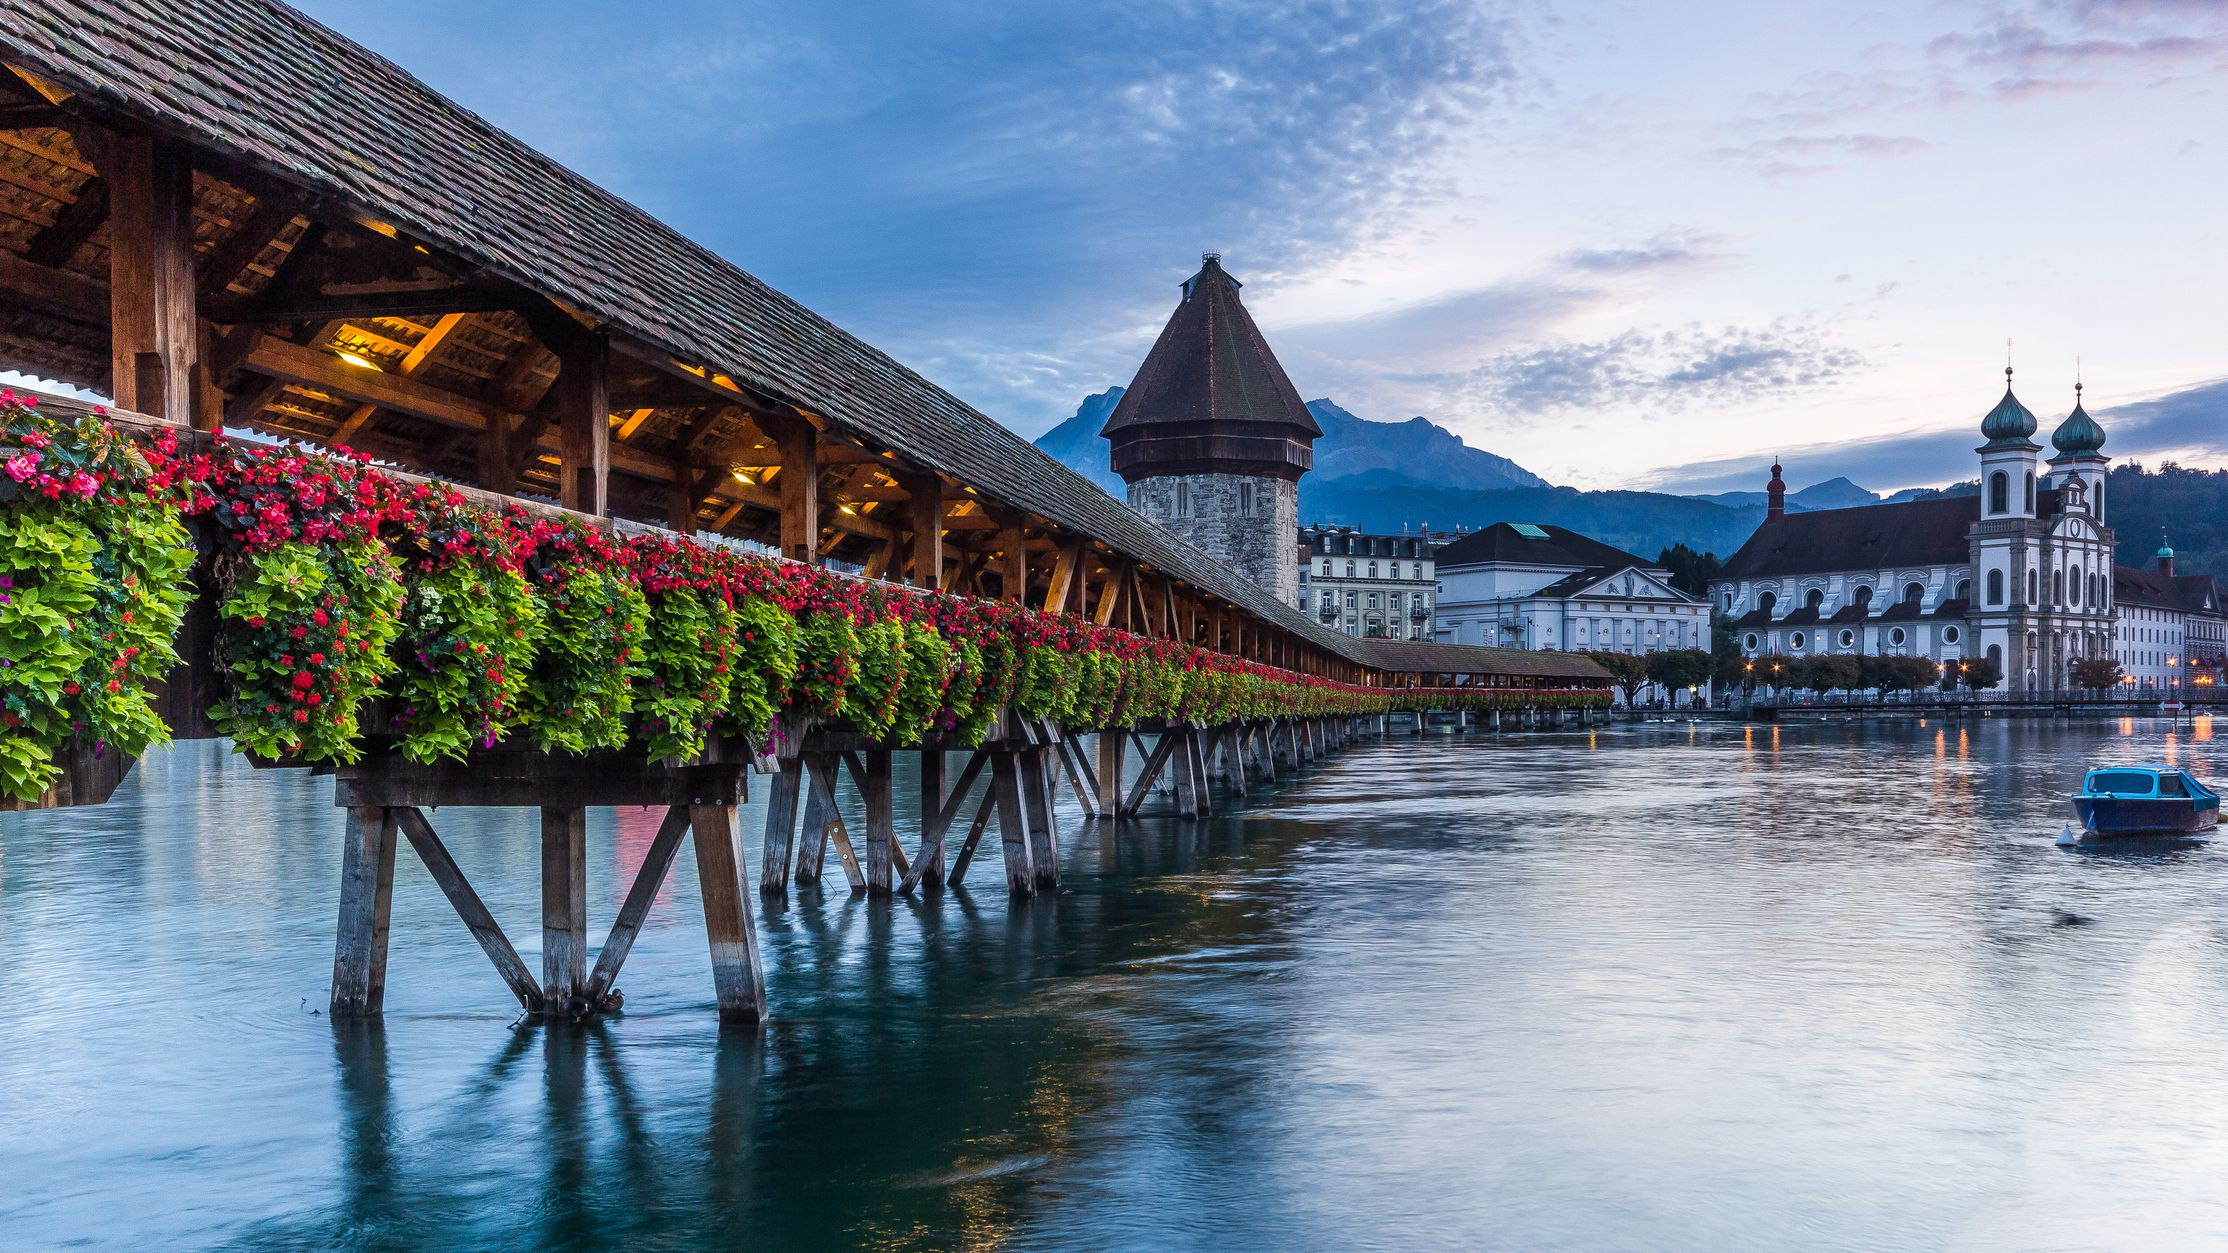
\includegraphics[width=0.95\linewidth]{../fig/placeholder}
		\caption{Bild rechts}
		\label{fig:right}
	\end{subfigure}
	\caption{Zwei Bilder nebeneinander}\label{fig:two_pictures}
\end{figure}\vspace{\skipAfterFigure pt}
{\footnotesize Quelle: \url{https://google.ch}, aufgerufen am 05.10.2019} 
\paragraph{Unterunterunterkapitel}
We have to go deeper.
\subsection{Weiteres Unterkapitel mit Tabelle}
\lipsum[1]
\begin{table}[H]\label{tab:table_description}
	\centering
	\caption{Tabellenbeschreibung}
	\begin{tabular}{|c|c|c|}
	\hline
  	\textbf{Methodik} & \textbf{Ermittelte Dehnung |\textit{$\epsilon$}|} & \textbf{Referenz}\\ \hline
  	a & \SI{720}{\micro\meter/\meter} & w \\ \hline
  	b & \SI{605.3}{\micro\meter/\meter} & x \\ \hline
  	c & \SI{655.77}{\micro\meter/\meter} & y \\ \hline
  	d & \SI{1247.10}{\micro\meter/\meter} & z \\ \hline
	\end{tabular}
\end{table}
\subsection{Weiteres Unterkapitel mit grosser Tabelle}
\begin{table}[H]
\centering
\caption{Eine etwas grössere Tabelle mit einer Spalte mit viel Text}\vspace{-3mm}
\begin{tabularx}{\textwidth}{|c|c|c|Y|}
\hline
\textbf{Modul/Funktion} & \textbf{Funktions-Detail} & \textbf{Status} & \textbf{Kommentar} \\ \hline
\multirow{4}{*}{\begin{tabular}[c]{@{}c@{}}Motorenkontroller \\ zur Ansteuerung \\ des DUT\end{tabular}} & Setzen digitaler Signale & OK & - \\ \cline{2-4} 
 & Einlesen digitaler Signale & OK & - \\ \cline{2-4} 
 & Ausgeben analoger Signale & NOK & Probleme mit DAC auf dem PCBA \\ \cline{2-4} 
 & Einlesen analoger Signale & OK & Abgleich der Nichtlinearität und Offset offen \\ \hline
\multirow{2}{*}{\begin{tabular}[c]{@{}c@{}}RHE zur Ansteuerung \\ der Hysteresebremse\end{tabular}} & Vorgabe Soll-Wert & NOK & Probleme mit DAC auf dem PCBA \\ \cline{2-4} 
 & Einlesen Ist-Wert & OK & Abgleich der Nichtlinearität und Offset offen \\ \hline
\begin{tabular}[c]{@{}c@{}}Druckmessung  \\ in Vakuumkammer\end{tabular} & Mit Varian FRG-700 & OK & Abgleich der Nichtlinearität und Offset offen \\ \hline
Temperaturmessung & Messung der Pt100 RTDs & OK & Genauigkeit verbesserungsfähig \\ \hline
Drehmomentmessung & Messen der DMS mittels WFB & N/A & Noch nicht getestet \\ \hline
\end{tabularx}
\end{table}
\textbf{Formel mit Nummerierung:}
\begin{equation}\label{equ:some_formula}
T = \dfrac{\sqrt{\left(A^2 \cdot R_0 - 4 \cdot B \cdot (-dR) \right) \cdot R_0} - A \cdot R_0}{2 \cdot B \cdot R_0} = \SI{0.0443}{\celsius}
\end{equation}
\textbf{Formel ohne Nummerierung:}\\
Elemente mit Labels können referenziert werden, wie beispielsweise die Formel \ref{equ:some_formula}.
\begin{equation*}
T = \dfrac{\sqrt{\left(A^2 \cdot R_0 - 4 \cdot B \cdot (-dR) \right) \cdot R_0} - A \cdot R_0}{2 \cdot B \cdot R_0} = \SI{0.0443}{\celsius}
\end{equation*}
\section{Zweites Hauptkapitel}
Beispiel für Pseudocode.\\
\begin{Verbatim}[tabsize=2,frame=single,label=Pseudo code of the firmware main-method,baselinestretch=0.8,numbers=left]
initialize all modules (of MC and peripherial)
allocate memory for test data buffers
seconds := 0 (timer-variable for logdata to be written to micro-sd-card)
DO ENDLESS:
	IF command received over over uart interface THEN
		execute command if it is valid
	END IF
	IF measurement due THEN
		toggle led to indicate start of measurement
		perform all measurements and create a string that contains all data
		IF values must be sent over uart THEN
			send all measurement values over uart
		END IF
		IF values must be written to micro sd card THEN
			write all values to the micro-sd-card
		END IF
	END IF	
	seconds := seconds + 1
REPEAT
\end{Verbatim}
\newpage
% einfacher Zeilenabstand

%------------------------------------------------------------------------------------------
% QUELLEN- UND LITERATURVERZEICHNIS
%------------------------------------------------------------------------------------------
\singlespacing
\rhead{\emph{Quellen- und Literaturverzeichnis}}
\bibliographystyle{apacite}
\bibliography{References}

%------------------------------------------------------------------------------------------
% ANHANG
%------------------------------------------------------------------------------------------
\newpage
\section{Anhang}
\appendix 
\rhead{\emph{Anhang}}
\renewcommand{\thesubsection}{\Alph{subsection}} % Anhänge einrücken

% Anhänge kommen hier hin
\subsection{Anhang 1}\label{apx:anhang1}


% leere Abschlussseite
%\newpage
%\thispagestyle{empty} % erzeugt Seite ohne Kopf- / Fusszeile
%\mbox{}
\end{document}